\documentclass{beamer}
\usepackage{amssymb, amsfonts, latexsym, amsthm, amsmath, framed}
\usepackage{esvect, parskip, amsmath, amssymb, framed, tcolorbox}
\usepackage{mathrsfs, xcolor, animate, graphicx}
\usepackage[backend=biber,style=numeric,sorting=none]{biblatex}
\setbeamerfont{footnote}{size=\tiny}
\addbibresource{ref.bib}
\tcbuselibrary{theorems}
\usepackage{listings}
\definecolor{green}{rgb}{0,0.6,0}
\definecolor{gray}{rgb}{0.5,0.5,0.5}
\definecolor{mauve}{rgb}{0.58,0,0.82}
\lstset{
    frame=none,
    language=Java,
    showstringspaces=false,
    columns=fullflexible,
    basicstyle = \ttfamily\small,
    numbers=none,
    numberstyle=\tiny\color{gray},
    keywordstyle=\color{blue},
    commentstyle=\color{green},
    stringstyle=\color{mauve},
    breaklines=true,
    morekeywords={function},
    breakatwhitespace=true,
    tabsize=4
}

% Beamer theme setting
\definecolor{myteal}{cmyk}{0.5,0,0.15,0}
\usecolortheme[named=myteal]{structure}
\definecolor{my-yellow}{cmyk}{0,0.2,0.7,0,1.00}
\definecolor{my-blue}{cmyk}{0.80, 0.13, 0.14, 0.04, 1.00}
\definecolor{my-green}{cmyk}{0.4,0,0.4,0,1.00}
\tcbset{
defstyle/.style={fonttitle=\bfseries\upshape, colback=my-yellow!5,colframe=my-yellow!80!black},
theostyle/.style={fonttitle=\bfseries\upshape, colback=my-blue!5,colframe=my-blue!80!black},
corstyle/.style={fonttitle=\bfseries\upshape, colback=my-green!5,colframe=my-green!80!black},
}
\usetheme{Madrid}
\setbeamertemplate{itemize items}[triangle]
\setbeamertemplate{enumerate items}[default]

% Title page
\title{Locke's Argument on Possibility of Material Mind}
\author{Ben Chen}
\institute{Dept of Computer Science and Engineering,\\ Southern University of Science and Technology}
\date{\today}

\begin{document}
\frame{\titlepage}
\begin{frame}
    \frametitle{How us be able to think?}
    \begin{columns}
        \begin{column}{0.6\textwidth}
            \centering
            Human beings think, but do they think because thinking is a power of their \textbf{material} body, or because there is an \textbf{immaterial} thinking part of them? \cite{locke-1700}
            \begin{itemize}
                \item<2-> We don't know which is the case.
                \item<3-> But Locke argues that the material mind is possible.
            \end{itemize}
        \end{column}
        \begin{column}{0.4\textwidth}
            \centering
            \animategraphics[autoplay, loop, width=.6\textwidth]{15}{img/moxiaba}{1}{110}
            
\includegraphics[width=.6\textwidth]{img/ruoyousuosi.jpg}
        \end{column}
    \end{columns}
\end{frame}

\begin{frame}
    \frametitle{Locke's argument on possibility of Material Mind}
    \begin{quote}
        It being, in respect of our notions, not much more remote from our comprehension to conceive, that God can, if he pleases, superadd to matter a faculty of thinking, than that he should superadd to it another substance with a faculty of thinking [...] since we know not wherein thinking consists, nor to what sort of substances the Almighty has been pleased to give that power.
        \par{\hfill-- \textit{An Essay Concerning Human Understanding}}
    \end{quote}
    \begin{block}{Argument for the possible material mind}
        \begin{enumerate}
            \item<1> God is perfect and omnipotent. $\phi$
            \item<1,2> If God is omnipotent, then he could superadd a faculty of thinking to matter,
            whatever the form of thinking is. $\phi \rightarrow \psi$
            \item<1> Therefore, it is possible for matter to think. $\psi$ [Modus Ponens]
        \end{enumerate}
    \end{block}
\end{frame}

\begin{frame}
    \frametitle{Is It Possible?}
    \centering
    Can the superaddition be possible? \\
    How is the superaddition done?
\end{frame}

\begin{frame}
    \frametitle{Stillingfleet against the Material Mind}
    \begin{small}
    \begin{quote}
    And here again you say, That the Power of Thinking joined to Matter, makes it a Spiritual Substance. But as to your Argument from God s Omnipotency, I answer, That this comes to the same Debate we had with the Papists about the Possibility of Transubstantiation. For, they never imagin'd, that a Body could be present after the manner of a Spirit in an ordinary way, but that by God's Omnipotent Power it might be made so: but our Answer to them was, That God doth not change the Essential Properties of things while the things themselves remain in their own Nature: And that it was as repugnant for a Body to be after the manner of a Spirit, as for a Body and Spirit to be the same. The same we say in this Case. We do not set bounds to God's Omnipotency: For he may if he please, change a Body into an Immaterial Substance; \textbf{but we say, that while he continues the Essential Properties of Things, it is as impossible for Matter to think, as for a Body by Transubstantiation to be present after the manner of a Spirit;} and we are as certain of one as we are of the other. \cite{stillingfleet-1698}
    \end{quote}
    \end{small}
\end{frame}

\begin{frame}
    \frametitle{TL;DR}
    \begin{block}{Argument against the Possibility of Material Mind}
        \begin{enumerate}
            \item God is omnipotent to change body into an immaterial thing with the essence of body remaining. $\phi$
            \item If matter can be transubstantiated into mind, then it is impossible for matter to think. $\phi \rightarrow \neg \psi$
            \item Therefore, it is impossible for matter to think. $\neg \psi$ [Modus Ponens]
        \end{enumerate}
    \end{block}
    \begin{block}{Implicit Attack}
        The superaddition is unnecessary and impossible.
    \end{block}
    Can substance be transubstantiated between material and immaterial? \\
    \emph{No, the matter cannot appear or disappear.}
\end{frame}

\begin{frame}
    \frametitle{Modern Interpretation}
    \begin{columns}
        \begin{column}{.6\textwidth}
            Karl Marx's materialism \cite{marx-1932}:
            \begin{itemize}
                \item Men's social beings determine their consciousness.
                \item Material comes primarily, consciousness secondarily.
            \end{itemize}
            Finding of the Brain Science:
            \begin{itemize}
                \item Mind is generated by neural cells.
                \item Mind is a product of material brain \\ $\Rightarrow$ material mind.
            \end{itemize}
            Modern mainstream view favors Locke's argument, i.e., material mind is possible.
        \end{column}
        \begin{column}{.4\textwidth}
            \centering
            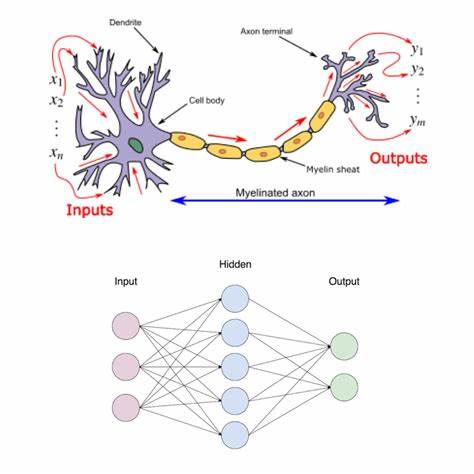
\includegraphics[width=1\textwidth]{img/nerual.jpeg}
        \end{column}
    \end{columns}
\end{frame}

\begin{frame}
    \frametitle{My Response}
    What if the Mind does not even exist?
    \begin{itemize}
        \item<2-> Our thoughts are just the result of the interaction of the material world. \emph{No, it is Naive Materialism.}
        \item<3-> The thinking matter is the representation of the Mind in the material world. \emph{Yes, and mind can be generated by matter.}
    \end{itemize}
\end{frame}

\begin{frame}[fragile]
    \frametitle{Analog of the Material Mind}
    How can the silicon turn into a running program?
    \begin{itemize}
        \item The program can be treated as a form of thinking, generated by the silicon. A simulation of our brain be like:
            \begin{lstlisting}
function Human() {
    while (alive()) { // check if the body is alive
        input();  // perceive the world
        think();  // generate idea and knowledge
        output(); // move or speak or play Genshin Impact
    }
    free(&mind);  // release the soul
}
            \end{lstlisting}
        \item<2-> People act as the God to make the silicon think.
        \item<3-> The electronic signal is the representation of the program(mind) in the material world.
    \end{itemize}
\end{frame}

\begin{frame}
    \frametitle{The Matrix}
    \centering
    {\large \emph{ Are we living in a simulation run by the computer? \\ Is Digital Life possible?}}
\end{frame}

\begin{frame}
    \frametitle{Q \& A}
    {\Huge \textbf{Q \& A}}
\end{frame}

\begin{frame}
    \frametitle{The END}
    \centering
    {\Huge \textbf{Thank you!}}
\end{frame}

\begin{frame}
    \frametitle{References}
    \printbibliography
\end{frame}

\end{document}
